% !TeX encoding = UTF-8
% !TeX program = xelatex
% !TeX spellcheck = en_US

\documentclass[degree=project,degree-type=project,cjk-font=noto]{thuthesis}
\usepackage{mathtools}
\usepackage{tikz}
\usetikzlibrary{shapes,arrows}
\usepackage[autosize]{dot2texi}
% Syntax Highlighting in LaTeX, need pygments
% Must build with xelatex -shell-escape -enable-8bit-chars.
\usepackage{minted}
% https://tex.stackexchange.com/a/112573
\usepackage{tcolorbox}
\usepackage{etoolbox}
\BeforeBeginEnvironment{minted}{\begin{tcolorbox}}%
\AfterEndEnvironment{minted}{\end{tcolorbox}}%
% color for minted
\definecolor{friendlybg}{HTML}{f0f0f0}


% 论文基本配置,加载宏包等全局配置
\thusetup{
    output = electronic,
    title  = {推荐系统},
    author  = {肖文韬},
    studentid = {2020214245},
    major = {电子信息(计算机技术)},
    email = {xwt20@xwt20@gmail.com},
    course = {大数据分析(B)},
    include-spine = false,
}

\usepackage{float}
\usepackage[sort]{natbib}
\bibliographystyle{thuthesis-numeric}
\graphicspath{{figures/}}

\begin{document}

% 封面
\maketitle

\frontmatter
\begin{abstract}
  点击率预测是推荐系统中的一项重要任务,其目的是估计用户点击某项目的概率,对许多在线应用(如在线广告)至关重要。
  推荐系统的数据来源的特点是多域(multi-field)数据,即数据由来源于许多不同域的特征组合而成(例如用户性别、年龄、浏览记录等)。
  这些多域数据的组合特征(combinatorial features)便是许多商业模式成功的必要条件。
  最近,许多深度模型被提出来从原始特征中学习低阶和高阶特征交互。

  \thusetup{
    keywords = {推荐系统, 点击率预测,深度学习, xDeepFM, AutoInt, FGCNN},
	}
\end{abstract}


% 目录
\tableofcontents

% 插图和附表清单
\listoffigures           % 插图清单

% 正文部分
\mainmatter

\chapter{任务一:Viterbi 解码算法实现}

Forward 和 Backward 算法对应于讲义中的 Q1 (Evaluation),Vertibi 算法对应于讲义中的 Q2 (Decoding)。
代码实现可以使用 \texttt{sanity\_grader\_hmm()} 测试是否正确。
算法的核心思路及实现如下:

\section{Forward 算法}
  输入:

  \begin{enumerate}
    \item $O$: observations
    \item $\pi$: initial probability
    \item $A$: hidden state transition matrix
    \item $B$: emission matrix
  \end{enumerate}

  输出:

  \begin{align}
    \begin{split}
      P(O | \lambda) &= \sum_{Q} P(O, Q | \lambda) \\
      &= \sum_Q P(O | Q, \lambda) P(Q | \lambda) \\
      &= \sum_Q \prod_{t=1}^T B(q_t, o_t) \pi(q_1) \prod_{t=2}^T A(q_{t-1}, q_t)
    \end{split}
    \label{algo_fwd}
  \end{align}

  公式 \ref{algo_fwd} 可以转换成矩阵运算:

  \begin{align}
    \begin{split}
      \pi^{(0)} &= \pi \\
      \text{Fwd}(o_1) &= \pi^{(1)} = \pi^{(0)} * B(:, o_1), P(o_1) = sum(\text{Fwd}(o_1)) \\
      &\vdots \\
      \text{Fwd}(o_1, \cdots, o_T) &= \pi^{(T)} = \pi^{(T-1)} * B(:, o_T) \\
      P(o_1, \cdots, o_T) &= sum(\text{Fwd}(o_1. \cdots, o_T))
    \end{split}
  \end{align}

  算法复杂度:$O(T * N^2)$

  实现代码:

  \begin{minted}[texcomments,tabsize=2,fontsize=\large,style=friendly,bgcolor=friendlybg]{python}
for t, o_t in enumerate(ob):
  fwd[t] = pi_t * B[:, o_t]
  pi_t = fwd[t] @ A
  \end{minted}


\section{Backward 算法}

Backward 算法目标与 Forward 一样,只不过迭代顺序是从后往前。
代码:

  \begin{minted}[texcomments,tabsize=2,fontsize=\large,style=friendly,bgcolor=friendlybg]{python}
beta_t = np.ones(total_states)
for t, o_t in enumerate(reversed(ob)):
  bwd[-1-t] = beta_t.T
  beta_t = A @ (B[:, o_t] * beta_t)
  \end{minted}

\section{Viterbi 算法}

目标:

启发式搜索 $Q^* = \arg \max_Q P(Q | O, \lambda)$:

\begin{align}
  \begin{split}
    Q^* &= \arg \max_Q P(Q | O, \lambda) \\
    &= \arg \max_Q P(Q, O | \lambda) / P(O | \lambda) \\
    &= \arg \max_Q P(Q, O | \lambda) \\
    &= \arg \max_Q P(O | Q, \lambda) P(Q | \lambda) \\
    &= \arg \max_Q \prod_{t=1}^T B(q_t, o_t) \pi(q_1) \prod_{t=2}^T A(q_{t-1}, q_t)
  \end{split}
  \label{algo_viterbi}
\end{align}

同样地,类似 Forward 算法,上式 \ref{algo_viterbi} 可以优化为迭代形式:

\begin{equation}
\delta_t (j) = \arg \max_{q_1, q_2, \cdots, q_{t-1}} P(q_1, \cdots, q_{t-1}, q_t=s_j, o_1, \cdots, o_t | \lambda)
\end{equation}

初始化:

\begin{equation}
  \delta_1 = \pi * B(:, o_1)
\end{equation}

递推式:

\begin{align}
  \begin{split}
    \phi_t &= \arg \max(\delta_{t-1} \odot A^T, \text{axis}=1) \\
    \delta_t &= \max(\delta_{t-1} \odot A^T, \text{axis}=1) * B(:, o_t)
  \end{split}
\end{align}

代码实现:

  \begin{minted}[texcomments,tabsize=2,fontsize=\large,style=friendly,bgcolor=friendlybg]{python}
delta_t = pi
phi_t = np.zeros(total_states)
for t, o_t in enumerate(ob):
  delta_t *= B[:, o_t]
  delta[t] = delta_t
  phi[t] = phi_t
  phi_t = np.argmax(delta_t * A.T, axis=1)
  delta_t = np.max(delta_t * A.T, axis=1)
  \end{minted}

\chapter{任务二:基于 GMM-HMM 的语音识别}

\section{Q1 ($3"$)}

Q: Look at the directory data/train, describe what is contained in files text, wav.scp and utt2spk respectively (Hint: all those files can be seen as key-value dicts).

A:

\begin{enumerate}
  \item text: 每一行地第一个元素是 utterance-id,可以为任意字符串。后面的部分就是每一句的录音对应的文本(字幕),如果有词不在字典中(out of vocabulary),将会自动映射到 data/lang/oov.txt 中指定的词。
  \item wav.scp:格式为 \texttt{<recording-id> <extended-filename>},extended-filename 可以为音频文件,也可以是能够返回出 wav 音频文件的任意命令。如果不存在 segments 文件,recording-id 就会自动用作 utterance-id。
  \item utt2sp: 每一行的格式为 \texttt{<utterance-id> <speaker-id>},用于标识每一个发音对应的发音者(speaker)。
\end{enumerate}

需要注意的有:

\begin{enumerate}
  \item 这些文件中的顺序需要对应起来
  \item wav.scp 中的音频文件必须是单通道的,否则需要用 sox 命令提取出指定的 channel。
  \item utterance-id, speaker-id 都推荐各自使用固定长度,否则可能回导致 C-style string order 出问题。
\end{enumerate}

\section{Q2 ($3"$)}

Q: Look at the file data/lang/topo, which contains two kinds of HMM topology, draw them using circles and arrows like this. You may notice that the HMM topology of a special phoneme is different from other phonemes. Use data/lang/phones.txt to map and find the name of the special phoneme.

\begin{figure}[h]
\centering%
  \begin{subfigure}{.85\linewidth}
    \begin{dot2tex}[dot,options=-tmath]
    digraph G1 {
      rankdir=LR;
      S_0 -> S_0 [label="0.75"];
      S_0 -> S_1 [label="0.25"];
      S_1 -> S_1 [label="0.75"];
      S_1 -> S_2 [label="0.25"];
      S_2 -> S_2 [label="0.75"];
      S_2 -> S_3 [label="0.25"];
   }
    \end{dot2tex}
    \caption{拓扑图 $1$ (real phonemes)}\label{fig:topo1}
  \end{subfigure}
\hspace{4em}%
  \begin{subfigure}{.85\linewidth}
    \begin{dot2tex}[dot,options=-tmath]
    digraph G2 {
      rankdir=LR;
      S_0 -> S_0 [label="0.5"];
      S_0 -> S_1 [label="0.5"];
      S_1 -> S_1 [label="0.5"];
      S_1 -> S_2 [label="0.5"];
      S_2 -> S_2 [label="0.75"];
      S_2 -> S_3 [label="0.25"];
   }
    \end{dot2tex}
    \caption{拓扑图 $2$ (silence and noise phonemes)}\label{fig:topo2}
  \end{subfigure}
  \caption{Q2 两种拓扑图}
  \label{fig:q2}
\end{figure}

A: data/lang/topo 中的两个 HMM 拓扑图如图 \ref{fig:q2} 所示,第二个拓扑图对应的是 \textbf{沉默和噪声音素(silence and noise phonemes)}。通过 topo 文件中的 \texttt{ForPhones} 字段(在本例中为 1),我们可以在 phones.txt 中找到对应的音素名称为 \texttt{sil}。

\section{Q3 ($2"$)}

Q: You can change num-sil-states and num-nonsil-states for command utils/prepare\_lang.sh in run.sh:line59, then run this stage again and draw new topologies from data/lang/topo. (Note that set them to default values(sil=3 and nonsil=3) and rerun this stage before proceeding to the next stage since other values may affect the performance).

\begin{figure}[h]
\centering%
  \begin{subfigure}{.85\linewidth}
    \begin{dot2tex}[dot,options=-tmath]
    digraph G1 {
      rankdir=LR;
      S_0 -> S_0 [label="0.75"];
      S_0 -> S_1 [label="0.25"];
      S_1 -> S_1 [label="0.75"];
      S_1 -> S_2 [label="0.25"];
   }
    \end{dot2tex}
    \caption{拓扑图 $1$ (real phonemes)}\label{fig:q3_topo1}
  \end{subfigure}
\hspace{4em}%
  \begin{subfigure}{.85\linewidth}
    \begin{dot2tex}[dot,options=-tmath]
    digraph G2 {
      graph [mindist=0.5];
      rankdir=LR;
      S_0 -> S_0 [label="0.33"];
      S_0 -> S_1 [label="0.33"];
      S_0 -> S_2 [label="0.33"];
      S_1 -> S_1 [label="0.33"];
      S_1 -> S_2 [label="0.33"];
      S_1 -> S_3 [label="0.33"];
      S_2 -> S_1 [label="0.33"];
      S_2 -> S_2 [label="0.33"];
      S_2 -> S_3 [label="0.33"];
      S_3 -> S_3 [label="0.75"];
      S_3 -> S_4 [label="0.25"];
   }
    \end{dot2tex}
    \caption{拓扑图 $2$ (silence and noise phonemes)}\label{fig:q3_topo2}
  \end{subfigure}
  \caption{Q3 修改参数后的两种拓扑图}
  \label{fig:q3}
\end{figure}

A: 将 \texttt{num-sil-states} 和 \texttt{num-nonsil-states} 分别修改为 $2$ 和 $4$,得到的对 real phonemes 和 silence and noise phonemes 的 HMM 的状态就会变为 $2$ 和 $4$。具体的拓扑图见图\ref{fig:q3}。

\section{Q4 ($7"$)}

Q: Describe the process of calculating MFCC, docs: link.

A: 首先从音频文件中提取出帧(frame),通常是 25ms 一帧,每次滑动 10ms。
然后对于每一帧:

\begin{enumerate}
  \item 提取数据,进行可选的预处理:抖动(dithering),预加权(preemphasis),dc 偏移消除(dc offset removal),最后乘以窗函数(例如 Hamming 窗)。
  \item 计算当前帧的能量(如果使用 log-energy 而不是 C0)
  \item 做快速傅立叶变换(FFT),计算能量谱(power spectrum)
  \item 计算每 mel bin 的能量,例如,23 个重叠矩形 bin,并且这些 bin 的中心点在 mel 频域上是等距的。频率的上下限一般取Nyquist频率(例如7800,对于16kHz采样的音频)和靠近0的频率(例如20)。
  \item 将这些能量取 log 然后进行余弦变换,保留指定数量(例如13)的系数 。
  \item 可选的倒谱提升(cepstral liftering),这就是将这些系数做一个缩放,保证它们在一个合理的范围内。
\end{enumerate}

\section{Q5 ($1"$)}

Q: Run following commands (Note: ark means archive file with binary format, ark,t means archive file with utf-8 text format), check file raw\_mfcc\_test.1.txt and answer the dimention of MFCC features. (Hint: count the number of columns)
  \begin{minted}[texcomments,tabsize=2,fontsize=\footnotesize,style=friendly,bgcolor=friendlybg]{bash}
source ./path.sh
copy-feats ark:mfcc/raw_mfcc_test.1.ark ark,t:raw_mfcc_test.1.txt
  \end{minted}

A: MFCC 特征共有 $13$ 个。

\section{Q6 ($1"$)}

Q: Look at the directory data/train, describe what is contained in file feats.scp, docs: link.

A: 每一行由 \texttt{<key> <rxfilename>:<byte\_offset>} 组成,其中 key 表示一个 utterance id, rxfilename 表示数据所在的文件名,byte\_offset 表示字节偏移量。

\section{Q7 ($1"$)}

Q: Describe the role of script utils/split\_scp.pl in steps/make\_mfcc.sh:line133. (Hint: type wc mfcc/raw\_mfcc\_train.1.scp and wc data/train/feats.scp, check the value of feats\_nj in run.sh and compare the outputs of the above commands)

A: 将 data/train/feats.scp 拆分为大致等长的 feats\_nj 个 scp 文件。

\section{Q8 ($1"$)}

Q: How many MonoPhones do we use ? (Hint: check exp/mono/phones.txt, the MonoPhones we mean here do not contain eps, \#0 and \#1)

A: $48$

\section{Q9 ($1"$)}

Q: If we choose 3-state HMM to model all those MonoPhones, how many states will we have ? (Hint: run the following commands and count the number of Triples in final.mono.mdl.txt)

  \begin{minted}[texcomments,tabsize=2,fontsize=\footnotesize,style=friendly,bgcolor=friendlybg]{bash}
source ./path.sh
gmm-copy --binary=false exp/mono/final.mdl final.mono.mdl.txt
  \end{minted}

A: $144$

\section{Q10 ($2"$)}

Q: According to the number of MonoPhones in the previous question, how many candidates are there for TriPhones and TriPhones' HMM states (suppose each HMM has 3 states) ?

A: 理论上需要 $48 \times 48 \times 48 = 110,592$ 个 TriPhones,并且需要 $110592 \times 3 = 331,776$ 个 HMM 状态。

\section{Q11 ($2"$)}

Q: Refer to Q9, use the correct command to view the TriPhone system (exp/tri1/final.mdl) and count the actual number of HMM states. You may find that the actual number of HMM states is much smaller than the theoretical value calculated in Q10, can you explain why ? (Hint: PPT5:page38~page42)

A: 使用命令 \texttt{gmm-copy --binary=false exp/tri1/final.mdl final.tri1.mdl.txt } 提取,TriPhone 的 HMM 实际上有状态为 $1929$ 个,远小于理论值。这是因为理论值太大,所以我们需要使用决策树来做一些聚类,\texttt{run.sh} 中的 \texttt{numLeavesTri1} (本例为 $2500$) 参数用于指定这个决策树的最大叶结点数。

\chapter{任务三:基于 DNN-HMM 的语音识别}

\section{Q1 ($1"$)}

Q: Explain what is force alignment. docs: link

A: 强制对齐(force alignment)是按照说话音频段对应文本,确定每一个出现的词对应与音频段中的具体时间。

\begin{figure}[h]
\centering%
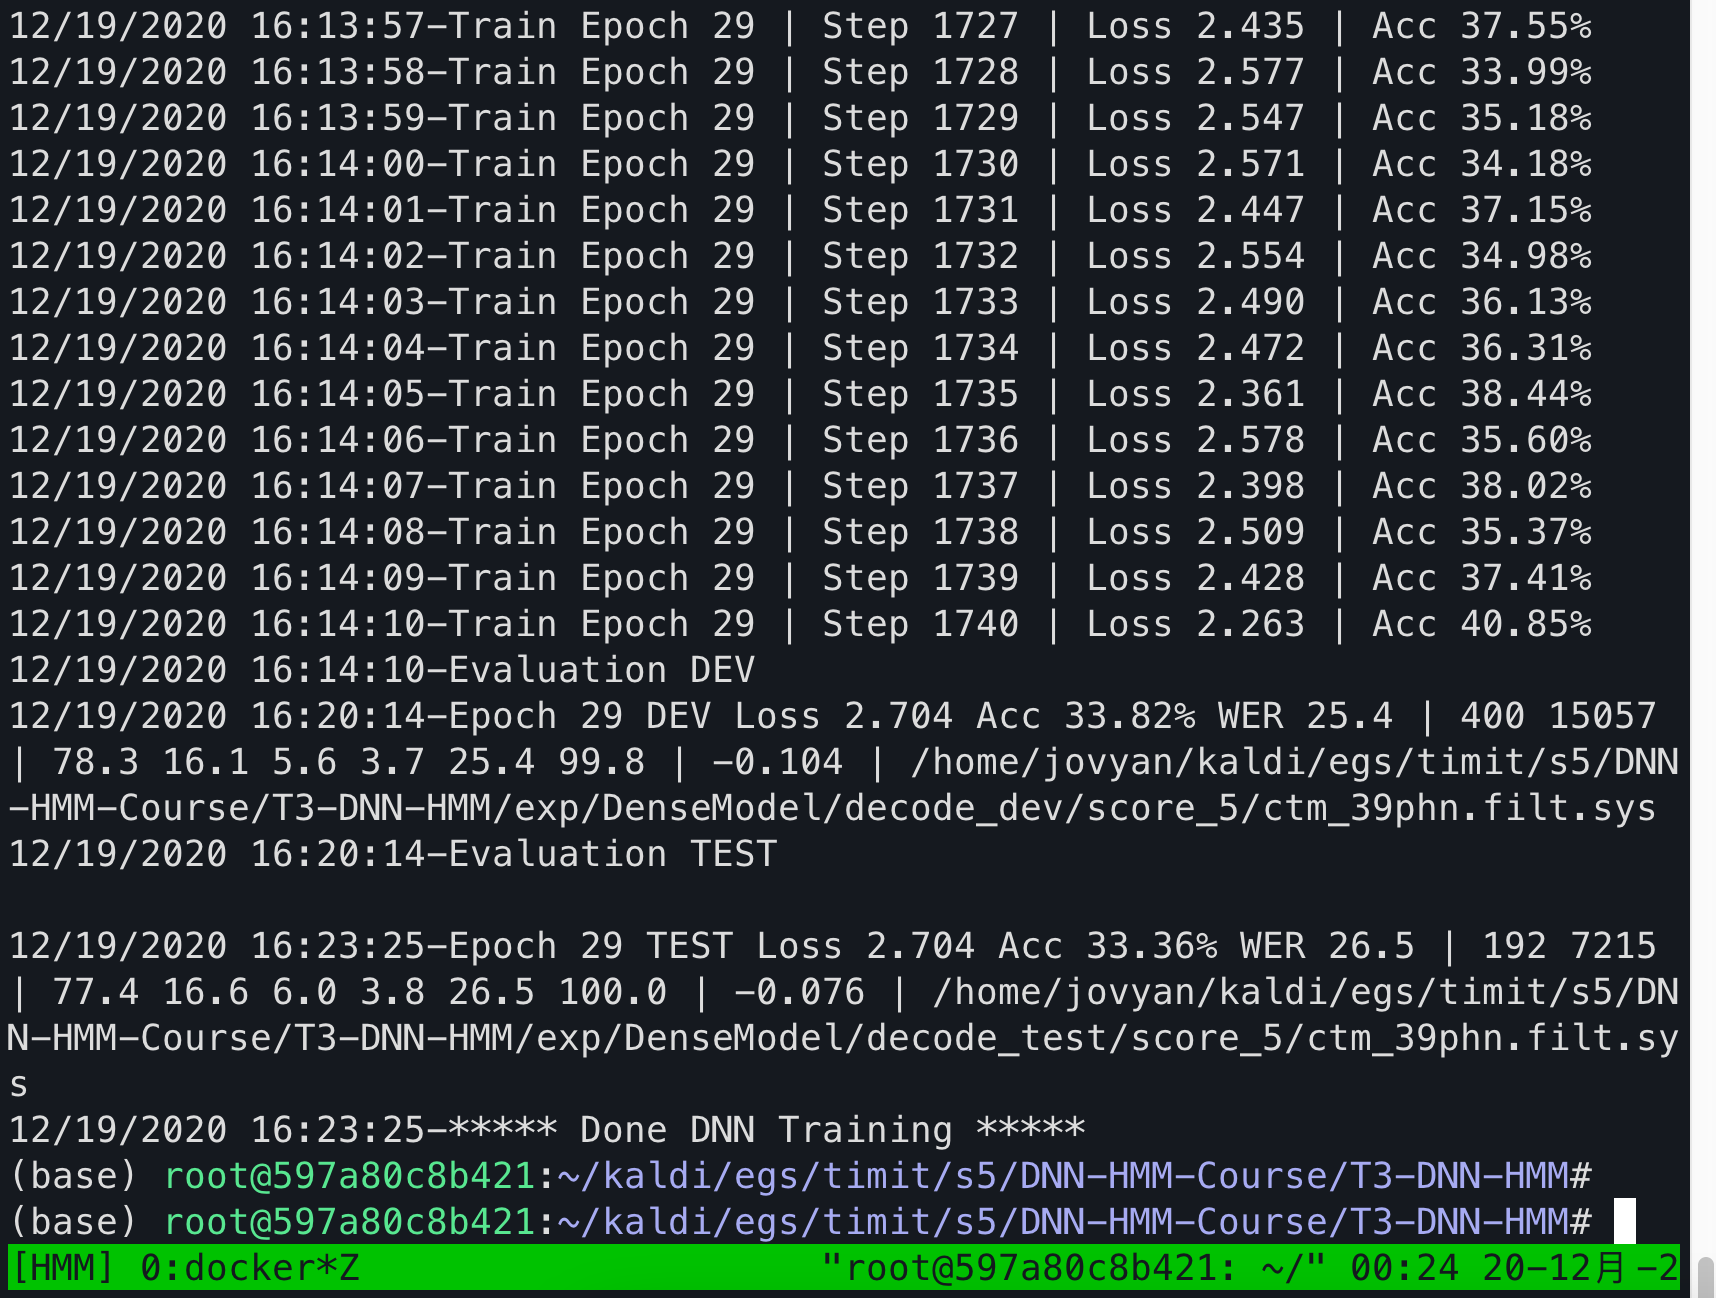
\includegraphics[width=.8\linewidth]{task3_dnn.png}
  \caption{DNN 训练结果}
  \label{fig:dnn}
\end{figure}

\section{Q2 ($1"$)}

Q: What is the dimention of transformed MFCC features ?

A: $39$

\section{Q3 ($2"$)}

Q: Explain why we need to subtract prior in train.py:line114-line115

A: 因为 $P(f1 | hh) = P(hh | f1) * P(f1) / P(hh)$,而 DNN 模型只能得到后验概率($P(hh | f1)$),我们需要除以 prior (先验概率)来得到似然概率($P(f1 | hh)$)。
取对数后除法就变成了减法了。

\section{DNN 实验结果}

训练 30 Epochs 后,得到 DEV 验证集结果为 \texttt{Acc 33.82\% WER 25.4},Test 测试集结果为 \texttt{Acc 33.36\% WER 26.5},如图 \ref{fig:dnn} 所示。

% 其他部分
\backmatter

% 参考文献
\bibliography{ref/refs}  % 参考文献使用 BibTeX 编译

% 附录
\appendix
\end{document}
